\documentclass[12pt]{article}
\usepackage{amsmath, amssymb}
\usepackage{geometry}
\geometry{a4paper, margin=1in}
\usepackage{parskip}
\usepackage{graphicx}
\usepackage{tikz}
\usetikzlibrary{shapes.geometric, arrows.meta}
\usepackage{enumitem}
\usepackage{booktabs}
\usepackage{hyperref}

\title{A Relativistic Theory of Longevity}
\author{Flyxion}
\date{\today}


\begin{document}

\maketitle

\begin{abstract}
The \textit{Relativistic Scalar--Vector Plenum} (RSVP) framework reconceives longevity as a state of recursive solvability within an entropic field system.  
Rather than opposing decay, enduring systems---biological, cognitive, or civilizational---persist by metabolizing entropy into structured potential.  
RSVP formalizes this process through three interacting fields: scalar capacity \((\Phi)\), vector flow \((\mathbf{v})\), and entropy density \((S)\), governed by a hepatic operator 
\(\mathcal{H}[\Phi,\mathbf{v},S]\) that enforces regenerative equilibrium.  
The condition \(\langle \mathcal{H} \rangle_\Omega \le 0\) defines the universal criterion for persistence: entropy must be reabsorbed faster than it accumulates.

Biologically, this principle manifests as the \textit{Hepastitium}---a distributed network of endothelial micro-robots and tomographic relays performing continuous, low-entropy self-repair and real-time entropy mapping.  
Cognitively, RSVP fields stabilize consciousness via low-entropy attractors that maintain identity continuity across morphological transformations.  
Architecturally, the same hepatic logic scales upward to \textit{xylomorphic} cities and ecological infrastructures that convert waste into regenerative flow, operationalizing sustainability as entropic coherence.  
Philosophically and ethically, longevity is reframed as the management of an entropic budget: the freedom to transform without decohering one’s recursive self.  
Civilizations, organisms, and minds alike persist through recursive hepatic operators that metabolize disorder into structure, aligning personal agency with reversibility and systemic integrity.

By unifying cosmological field theory, biomedical engineering, architecture, and philosophical recursion, RSVP proposes a relativistic theory of longevity grounded in continuous entropic descent.  
Life, in this view, endures not by resisting change but by falling outward through perpetual repair---a dynamic equilibrium in which energy, information, and identity remain coherently solvable across scales.

\textbf{Keywords:} RSVP theory; Hepastitium; longevity; entropy management; morphological agency; xylomorphic architecture; cognitive anti-senescence.
\end{abstract}


\subsection{Introduction}
\label{subsec:introduction}

The quest for longevity has historically been framed as a battle against entropy, drawing on thermodynamic principles articulated by Clausius and Boltzmann, and later reframed by Prigogine’s dissipative structures, which emphasized self-organization in far-from-equilibrium systems \cite{prigogine1977}. Schrödinger’s seminal question, “What is Life?”, posited life as a negentropic process, extracting order from environmental chaos \cite{schrodinger1944}. Contemporary longevity paradigms—genetic engineering, cellular therapies, cryonics, or AI consciousness uploads—often resist entropy through localized interventions, failing to address systemic recursion across scales. The Relativistic Scalar–Vector Plenum (RSVP) theory offers a novel framework, positing longevity as the recursive solvability of entropic challenges, where systems endure by internalizing mechanisms to metabolize disorder into structured potential.

At the heart of RSVP lies a triadic field structure: scalar capacity (\(\Phi\)), representing informational potential; vector flow (\(\mathbf{v}\)), denoting directed resource or agent transport; and entropy field (\(S\)), quantifying disorder. These fields, governed by coupled differential equations, unify cosmological, biological, architectural, and cognitive dynamics under a single entropic recursion law:
\begin{equation}
\langle \mathcal{H}[\Phi, \mathbf{v}, S] \rangle_\Omega \le 0,
\label{eq:hepatic_operator}
\end{equation}
where \(\mathcal{H}\) is the hepatic operator enforcing negentropic equilibrium over domain \(\Omega\). The Hepastitium, an endogenous biological network, exemplifies this principle, transforming the body into a self-observing, self-repairing plenum. This chapter explores how RSVP enables longevity across scales, from cellular maintenance to urban metabolism and cognitive persistence, redefining endurance as a recursive dialogue with entropy.

\section{RSVP Field Dynamics}
\label{sec:rsvp_dynamics}

The RSVP framework models reality as a plenum of interacting fields, ensuring coherence through recursive entropy management.

\subsection{Scalar Field \(\Phi\): Capacity}
\label{subsec:scalar_field}

The scalar field \(\Phi\) quantifies local informational or functional capacity, evolving via:
\begin{equation}
\frac{d\Phi}{dt} = -\nabla \cdot (\mathbf{v} \Phi) + \lambda (S_c - S) + \sum_k \alpha_k \delta \Phi_k.
\label{eq:phi_dynamics}
\end{equation}
Here, \(-\nabla \cdot (\mathbf{v} \Phi)\) represents the transport of capacity through vector flows, analogous to convective energy transfer. The term \(\lambda (S_c - S)\) acts as an entropic feedback control, correcting deviations from a critical entropy threshold \(S_c\). The summation \(\sum_k \alpha_k \delta \Phi_k\) incorporates intentional perturbations, such as microsurgical interventions in the Hepastitium, reflecting agent-like actions that enhance local vitality.

\subsection{Vector Field \(\mathbf{v}\): Flow}
\label{subsec:vector_field}

The vector field \(\mathbf{v}\) models directed flows of resources, information, or agents:
\begin{equation}
\frac{d\mathbf{v}}{dt} = -\nabla \Phi - \beta (\mathbf{v} \cdot \nabla) \mathbf{v} + \xi \nabla S.
\label{eq:v_dynamics}
\end{equation}
The gradient \(-\nabla \Phi\) couples flow to capacity gradients, \(-\beta (\mathbf{v} \cdot \nabla) \mathbf{v}\) introduces nonlinear advection, and \(\xi \nabla S\) drives adjustments based on entropy gradients, ensuring dynamic responsiveness.

\subsection{Entropy Field \(S\): Disorder}
\label{subsec:entropy_field}

The entropy field \(S\) balances coherence and chaos:
\begin{equation}
\frac{dS}{dt} = \kappa \nabla^2 S - \sum_k \gamma_k \Delta S_k.
\label{eq:s_dynamics}
\end{equation}
The diffusive term \(\kappa \nabla^2 S\) stabilizes entropy spatially, while \(-\sum_k \gamma_k \Delta S_k\) accounts for reductions from targeted interventions, such as microsurgical entropy clearance.

\subsection{Coupling and Hepatic Equilibrium}
\label{subsec:coupling}

The fields interact recursively, with perturbations in \(S\) altering \(\mathbf{v}\), which in turn modifies \(\Phi\). This coupling is visualized in Figure \ref{fig:field_coupling}, illustrating feedback loops that stabilize systemic dynamics.

\begin{figure}[h]
\centering
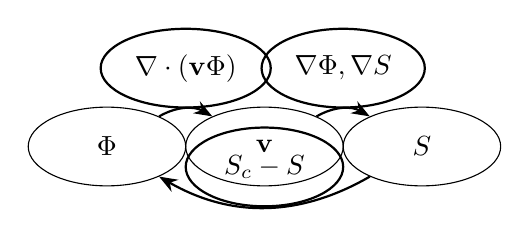
\begin{tikzpicture}[
  node distance=2cm,
  every node/.style={draw, ellipse, minimum height=1cm, minimum width=2cm, align=center},
  arrow/.style={-Stealth, thick}
]
\node (phi) {$\Phi$};
\node (v) [right of=phi] {$\mathbf{v}$};
\node (s) [right of=v] {$S$};
\draw[arrow] (phi) to [bend left] node[midway, above] {$\nabla \cdot (\mathbf{v} \Phi)$} (v);
\draw[arrow] (v) to [bend left] node[midway, above] {$\nabla \Phi, \nabla S$} (s);
\draw[arrow] (s) to [bend left] node[midway, above] {$S_c - S$} (phi);
\end{tikzpicture}
\caption{Coupling of RSVP fields, showing transport and feedback interactions.}
\label{fig:field_coupling}
\end{figure}

The hepatic operator \(\mathcal{H}[\Phi, \mathbf{v}, S]\) enforces negentropic equilibrium:
\begin{equation}
\langle \mathcal{H} \rangle_\Omega \le 0,
\label{eq:hepatic_equilibrium}
\end{equation}
acting as a Lyapunov-like functional whose negative time derivative ensures stability. A simple energy functional, \(E = \frac{1}{2} |\mathbf{v}|^2 + V(\Phi, S)\), with potential \(V\), satisfies \(\frac{dE}{dt} \propto \langle \mathcal{H} \rangle_\Omega\), confirming that longevity requires continuous entropic relaxation.

\section{Biological Longevity: The Hepastitium}
\label{sec:hepastitium}

The \emph{Hepastitium}, derived from Greek \emph{hepar} (liver) and Latin \emph{stitium} (standing-place or structure), denotes an endogenous, distributed network for continuous tissue maintenance and entropic regulation.  
It extends the regenerative role of the liver to every organ system, transforming the entire organism into a recursive hepatic field.  
Within the Relativistic Scalar--Vector Plenum (RSVP) framework, the Hepastitium operationalizes longevity as sustained entropic solvability: the capacity to metabolize disorder into structured potential through distributed microsurgery and continuous field sensing.

\subsection{Mechanisms}
\label{subsec:hepastitium_mechanisms}

The Hepastitium integrates hardware, software, and informational layers into a coherent recursive feedback network:

\begin{itemize}
  \item \textbf{Tomographic Relays:} Low-intensity X-ray, ultrasound, and terahertz arrays provide noninvasive, full-body imaging at cellular resolution.  
  Each voxel is mapped to its local entropy density \(S(x,y,z,t)\), producing a continuously updated four-dimensional entropy field.  
  Reconstruction pipelines employ compressive sensing and Bayesian inference to minimize radiation exposure while maintaining spatial precision.  
  These relays act as the sensory organs of the hepatic network, analogous to proprioception for the body’s internal thermodynamics.

  \item \textbf{Microsurgical Robots:} Millions of sub-millimeter endothelial agents operate within the vascular system, guided by RSVP’s scalar and vector fields.  
  Each robot executes targeted interventions such as plaque clearance, synaptic modulation, or DNA repair.  
  Their activity follows the scalar capacity equation:
  \begin{equation}
  \frac{d\Phi}{dt} = -\nabla\!\cdot(\mathbf{v}\Phi) + \lambda(S_c - S) + \xi\,\mathcal{H}[\Phi,\mathbf{v},S],
  \label{eq:phi_dynamics}
  \end{equation}
  ensuring that each local operation contributes to restoring systemic coherence rather than isolated correction.  
  The network’s coordination emerges through shared entropic gradients—microsurgeries collectively optimize the global condition \(\langle \mathcal{H} \rangle_\Omega \le 0\).

  \item \textbf{Morphological Agency:}  
  The same microsurgical infrastructure enables macroscopic, reversible transformations—height modulation through osteogenic scaffold elongation, limb reshaping via perfusion control, or body resizing through temporary metabolic reprogramming.  
  RSVP ensures that such changes occur within stable phase-space trajectories of \((\Phi, \mathbf{v}, S)\), preserving the continuity of consciousness and mechanical balance.  
  Morphology becomes a parameter of recursion rather than a fixed constraint.
\end{itemize}

Together, these components transform medicine from a reactive intervention to a continuous field discipline.  
The Hepastitium maintains equilibrium by sustaining the body as a distributed, self-reflective manifold—an organismic plenum engaged in ongoing entropic correction.

\subsection{Evolutionary Analogy}
\label{subsec:evolutionary_analogy}

The Hepastitium constitutes an evolutionary threshold: a transition from stochastic cellular maintenance to deliberate, recursive optimization.  
Natural biology relies on probabilistic micro-repairs—apoptosis, autophagy, immune pruning—where each event occurs locally and blindly, guided by statistical survival rather than global coherence.  
In contrast, the Hepastitium implements a deterministic feedback system informed by global entropy gradients and semantic causality.  
This parallels the shift from Darwinian selection to Lamarckian adaptation: a movement from passive fitness filtering to active structural learning.

From an evolutionary thermodynamic perspective, the Hepastitium extends the logic of endosymbiosis—where mitochondria internalized energy production—into the realm of repair and regulation.  
The organism internalizes its own maintenance infrastructure, creating an internal civilization of negentropic agents operating under the RSVP field laws.  
Entropy is no longer resisted but metabolized; disorder becomes fuel for structure.

\subsection{Energetic and Informational Constraints}
\label{subsec:hepastitium_constraints}

To remain physiologically viable, the Hepastitium must satisfy strict energy and information budgets.  
If each microsurgical event consumes energy \(\epsilon_i\) and reduces entropy by \(\Delta S_i\), the daily negentropic balance condition is:
\begin{equation}
\sum_i \epsilon_i \le E_{\mathrm{budget}}, \qquad 
\sum_i \Delta S_i \ge -\eta_{\mathrm{target}},
\end{equation}
where \(E_{\mathrm{budget}}\) denotes total metabolic energy available for maintenance and \(\eta_{\mathrm{target}}\) defines the desired entropy reduction threshold.  
This ensures that hepatic operations remain energy-neutral at the organismal scale.  
Information throughput is bounded by a recursive Shannon limit:
\begin{equation}
I_{\max} = \frac{E_{\mathrm{budget}}}{k_B T \ln 2},
\end{equation}
linking thermodynamic efficiency to informational capacity and defining a quantitative ceiling for daily microsurgical data exchange.

\subsection{Functional Summary}
\label{subsec:hepastitium_summary}

In total, the Hepastitium transforms the organism into a living computation of its own entropy field.  
Every cellular fluctuation becomes a data point in a recursive optimization process; every repair, a computation that preserves coherence.  
Longevity thus ceases to be the extension of lifespan and becomes the continuous redefinition of structure within solvable entropy bounds.  
The organism does not survive \emph{in} time—it survives \emph{through} time, by maintaining recursive compatibility between its scalar, vector, and entropy fields.

\begin{quote}
\emph{The Hepastitium is the body’s equation of persistence—its proof that life endures not by resisting decay but by learning how to metabolize it.}
\end{quote}
\subsection{Energy Economics}
\label{subsec:energy_economics}

Continuous microsurgical operation within the Hepastitium demands a stable energetic substrate.
Preliminary modeling suggests that maintaining millions of microsurgeries per day would consume approximately
10--20\% of the basal metabolic rate, depending on the efficiency of robotic circulation and data processing.
Such a load is sustainable only if the energetic cost of intervention is offset by a proportional reduction in
systemic entropy.

Within the RSVP framework, each micro-operation carries both an energy term \(\epsilon_i\) and an entropic return
\(\Delta S_i\). The effective efficiency \(\eta_{\mathrm{eff}}\) of the Hepastitium can thus be expressed as:
\begin{equation}
\eta_{\mathrm{eff}} = \frac{-\sum_i \Delta S_i}{\sum_i \epsilon_i / (k_B T)},
\end{equation}
representing the entropy reduction per thermodynamic bit of energy expended.  
Optimal function requires that \(\eta_{\mathrm{eff}} \geq \eta_{\mathrm{min}}\), the minimal efficiency ensuring
\(\langle \mathcal{H} \rangle_\Omega \le 0\), that is, net negentropic operation.

RSVP balances these metabolic costs by distributing hepatic effort according to the local entropy gradient:
\[
\mathbf{v}_{\mathcal{H}} = -\nabla S / \|\nabla S\|,
\]
ensuring that energy allocation favors regions with maximal disorder but high repair leverage.
In this sense, the Hepastitium performs a thermodynamic arbitrage: it converts ATP expenditure into informational
structure, maintaining \(S < S_c\) as defined by Equation~\eqref{eq:s_dynamics}.
Over time, the optimization of this balance may yield new metabolic regimes in which energy and information are
co-allocated, redefining the concept of nutritional intake as informational ingestion.

\subsection{Knowledge Infrastructure}
\label{subsec:knowledge_infrastructure}

Medical knowledge under the Hepastitium paradigm must be reorganized around entropy dynamics rather than static
disease taxonomies.  Instead of categorizing by pathology (\emph{what is wrong}), the new epistemic architecture
categorizes by \emph{entropic function} (\emph{how disorder propagates or is absorbed}).  This transforms medicine
into a recursive, explorable information system governed by feedback loops and causal inference.

Let \(\mathcal{G} = (V,E)\) denote the medical knowledge graph.  
Each node \(v_i \in V\) corresponds to a measurable entity or operator---a field variable
(\(\Phi,\mathbf{v},S\)) or micro-procedure---and each edge \(e_{ij} \in E\) encodes a causal relationship with
weight \(w_{ij}\) proportional to inferred entropic efficiency.  
The graph evolves through continuous learning as new data from tomographic relays and microsurgical outcomes
modify edge weights according to observed entropy changes.

\begin{verbatim}
function updateGraph(G, delta_S):
    for node in G.nodes:
        if node.type == "entropy" and node.value > S_c:
            for edge in G.edges(node):
                edge.weight += computeCausalInference(delta_S, edge)
    return G
\end{verbatim}

This pseudocode illustrates the recursive update cycle of the \emph{semantic microscope}, a software layer that
monitors entropy gradients and refines causal structure in real time.  
Each iteration constitutes an act of learning: local entropy excess triggers a search for correlated variables,
and edge weights are adjusted by the inferred magnitude of causal influence.  
The resulting network forms a continuously self-correcting epistemology---a living map of the organism’s
negentropic topology.

Practically, this allows medical exploration through recursive queries such as:
\begin{itemize}
  \item Identify all procedures where \(\Delta S / \epsilon > \eta_{\mathrm{min}}\);
  \item Trace causal chains reducing entropy in cardiac tissue by more than 5\%;
  \item Predict emergent regions of disorder by extrapolating entropy gradients along high-weight edges.
\end{itemize}

The semantic microscope thus transforms medical reasoning into a navigable, computational landscape:  
diagnosis becomes the identification of entropic attractors, and treatment the reconfiguration of causal flow
to restore regenerative equilibrium.

\subsection{Ethical Reflection}
\label{subsec:ethical_reflection}

Morphological adaptations---including height modulation, body resizing, or organ-level reconfiguration---introduce profound ethical questions regarding identity, autonomy, and continuity.  
Within the RSVP framework, these questions are not external to biology but intrinsic to its recursive coherence: identity itself is a function of stability in the coupled fields \((\Phi, \mathbf{v}, S)\).  
If the scalar capacity \(\Phi\) remains continuous and its divergence-free flows preserve entropy gradients within acceptable bounds, the system---biological or cognitive---maintains its phenomenological identity even as its morphology transforms.

The \emph{Hepastitium} therefore serves as both a biomedical and an ethical architecture.  
By anchoring all transformations within RSVP’s invariant coherence condition,
\[
\frac{d}{dt}\int_{\Omega} \Phi\, dV = 0 \quad \text{and} \quad 
\langle \mathcal{H} \rangle_\Omega \le 0,
\]
it guarantees that any morphological change respects informational conservation.  
In practical terms, this means that agency over form must be exercised through reversible, low-entropy operations, ensuring that the individual’s causal continuity---their experiential thread---remains unbroken across configurations.

Autonomy, in this context, is redefined as the freedom to transform without decohering.  
The right to self-modification thus coexists with a responsibility to maintain recursive solvability: a bioethical equilibrium between plasticity and persistence.  
This reversibility criterion replaces the older dichotomy of “natural versus artificial” with a gradient of coherence---any transformation is permissible so long as it remains entropically consistent with the system’s self-model.

At the societal level, the same principle extends to questions of enhancement, replication, and continuity across substrates.  
Cloning, uploading, or distributed embodiment may all preserve moral and personal identity if the hepatic operator maintains entropic coherence across the transition.  
The boundary of the self becomes not the skin, but the closure of negentropic recursion: the informational domain within which \(\Phi, \mathbf{v}, S\) remain jointly solvable.

Ultimately, the Hepastitium reframes bioethics as the geometry of reversible transformation.  
It replaces static ideals of form and purity with dynamic constraints of coherence and feedback.  
Longevity, in this sense, becomes a moral as well as biological pursuit: the commitment to remain integrable within the plenum of life, preserving one’s recursive role in the larger entropic economy.

\section{Architectural Extensions: Xylomorphic Designs}
\label{sec:xylomorphic_designs}

The hepatic logic of the Hepastitium extends to urban and ecological systems through xylomorphic designs, inspired by forest feedback loops.

\subsection{Xylomorphic Metabolism}
\label{subsec:xylomorphic_metabolism}

Cities emulate biological homeostasis, with waste cycles mirroring tree respiration and soil networks. Data centers, as metabolic hubs, process informational entropy, redirecting waste energy into regenerative structures, governed by:
\begin{equation}
E_{\mathrm{waste}} \rightarrow Q_{\mathrm{usable}},
\label{eq:work_heat}
\end{equation}
where \(E_{\mathrm{waste}}\) is dissipative energy and \(Q_{\mathrm{usable}}\) is redirected for environmental stability.

\subsection{Case Study: Hepatic City Block}
\label{subsec:city_block}

A city block functions as a hepatic module, with sensors detecting entropy gradients (e.g., waste accumulation) and Yarncrawler agents repairing infrastructure. Vector flows (\(\mathbf{v}\)) optimize resource distribution, ensuring negentropic balance akin to biological nutrient cycling.

\subsection{Philosophical Statement}
\label{subsec:architectural_philosophy}

Architecture becomes biomedicine scaled to civilization, where urban systems metabolize entropy to sustain ecological and social coherence, extending longevity to collective scales.

\section{Cognitive Anti-Senescence}
\label{sec:cognitive_anti_senescence}

RSVP fields stabilize consciousness through low-entropy attractors, preserving identity across substrate transitions.

\subsection{Mechanisms}
\label{subsec:cognitive_mechanisms}

Low-entropy attractors, visualized as minima in an energy landscape (Figure \ref{fig:energy_landscape}), stabilize neural dynamics. Semantic merge operators ensure continuity during memory reconsolidation, drawing on predictive coding and free-energy minimization principles \cite{friston2010}.

\begin{figure}[h]
\centering
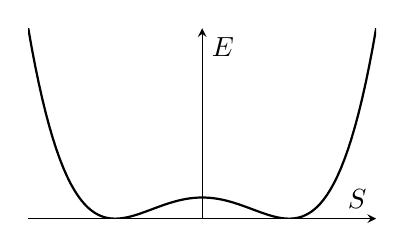
\begin{tikzpicture}
\begin{axis}[
    axis lines=middle,
    xlabel={$S$},
    ylabel={$E$},
    xtick=\empty, ytick=\empty,
    width=6cm, height=4cm
]
\addplot[domain=-2:2, samples=100, thick] {x^4 - 2*x^2 + 1};
\node at (axis cs:-1,-0.5) {Attractor};
\end{axis}
\end{tikzpicture}
\caption{Energy landscape with low-entropy attractors stabilizing cognitive states.}
\label{fig:energy_landscape}
\end{figure}

\subsection{Analogies to Biological Processes}
\label{subsec:cognitive_analogies}

\begin{table}[h]
\centering
\begin{tabular}{ll}
\toprule
\textbf{Biological} & \textbf{Cognitive} \\
\midrule
Cell regeneration & Memory reconsolidation \\
Enzyme repair & Conceptual re-weighting \\
Entropy clearance & Noise filtering \\
\bottomrule
\end{tabular}
\caption{Parallels between biological and cognitive hepatic processes.}
\label{tab:analogies}
\end{table}

These parallels highlight how RSVP dynamics unify physical and informational longevity.

\section{Philosophical Implications}
\label{sec:philosophical_implications}

The RSVP framework redefines persistence as indefinite renewal through information flow, resonating with Ortega y Gasset’s vital reason and Spinoza’s conatus \cite{ortega1930, spinoza1677}. The Hepastitium’s etymology—\emph{hepar} (regeneration) and \emph{stitium} (structure)—mirrors RSVP’s cosmological philosophy: every system has a “liver,” an interface where disorder is transmuted into meaning. Longevity is not immortality but recursive solvability, transforming entropy into a substrate for coherence.

\section{Empirical Validation}
\label{sec:empirical_validation}

The Relativistic Scalar--Vector Plenum (RSVP) framework and its associated
biomedical instantiation, the Hepastitium, yield specific, falsifiable
predictions across computational, biological, and cognitive domains.
Each prediction derives from measurable entropic dynamics and can be
expressed as a test of the regenerative equilibrium condition
\(\langle \mathcal{H} \rangle_\Omega \le 0\).
Validation therefore requires observing whether real systems maintain
persistent negentropic flux under controlled perturbation.

\subsection{Simulation Validation}

The simulation domain offers the most immediate route to empirical
exploration.  The turn-based strategy simulation
\emph{RSVP Economics: Entropic Empire} functions as a computational
analogue of the Hepastitium, embedding the field equations
(\(\Phi,\mathbf{v},S\)) in a discretized environment.
Each simulated world evolves according to
\begin{equation}
\Phi_{t+1} = \Phi_t - \nabla\!\cdot(\mathbf{v}_t \Phi_t)
  + \lambda (S_c - S_t) + \xi\,\mathcal{H}_t,
\end{equation}
where stability of the empire corresponds to satisfaction of the
longevity condition.  Empirical tests consist of measuring the
mean-field entropy flux and verifying that simulated civilizations
persist only when global \(\langle \mathcal{H} \rangle_\Omega < 0\).
This provides a quantitative sandbox for exploring entropic governance,
negentropic economics, and cross-scale feedback between local and
global equilibrium.

Agent-based extensions of the simulation can model Hepastitium-like
microsurgical agents as individual entities maintaining local
\(\Phi\)-gradients, enabling comparative studies between stochastic
(self-organizing) and coordinated (recursive) repair dynamics.  The
statistical lifetime of simulated structures serves as a direct proxy
for empirical longevity.

\subsection{Biomedical Validation}

Biological systems permit direct testing of RSVP's negentropic
hypothesis.  The Hepastitium predicts that continuous microscopic repair
should correlate with measurable reductions in entropy production and
improvements in structural order.

\begin{enumerate}[label=(\alph*)]
  \item \textbf{Entropy Production Rate (EPR):}
        Measure EPR in cultured tissues using microcalorimetry or
        flux-balance metabolic analysis.  The theory predicts that
        successful hepastitial interventions lower EPR while maintaining
        total energy throughput, indicating increased informational
        efficiency rather than energy suppression.
  \item \textbf{Mitochondrial Order Parameter:}
        Using super-resolution fluorescence or cryo-electron tomography,
        quantify mitochondrial cristae organization and membrane
        potential variability.  RSVP predicts that hepatic repair
        processes increase structural coherence—reflected by higher
        order parameters and reduced spatial entropy.
  \item \textbf{In Situ Negentropic Imaging:}
        Low-dose phase-contrast or terahertz tomography can generate
        voxelwise entropy maps of tissues.  Real-time observation of
        localized entropy reduction following micro-intervention would
        constitute direct validation of Equation~(4).
\end{enumerate}

Temporal analyses of these metrics should show that the integrated
entropy field,
\(\int_\Omega S(t)\, dV\), decreases monotonically during sustained
hepastitial activity and rebounds when the process is paused—demonstrating
reversible control of entropy flux.

\subsection{Cognitive Validation}

At the cognitive scale, RSVP predicts that conscious stability arises
from the formation of low-entropy attractors in neural field space.
Empirical verification requires correlating entropy measures of neural
activity with subjective continuity and attentional coherence.

\begin{itemize}
  \item \textbf{Neurodynamic Entropy:}
        Compute multiscale entropy (MSE) or permutation entropy of EEG or
        fMRI time series.  RSVP predicts a regime of intermediate entropy
        (neither minimal nor maximal) corresponding to maximal
        \(\Phi\)-coherence.
  \item \textbf{\(\Phi\)-Coherence Index:}
        Define \(\Phi_c = 1 - \frac{\mathrm{Var}(\Phi_i)}{\langle
        \Phi_i\rangle}\), where \(\Phi_i\) represents regional energy or
        functional capacity inferred from neural activation.
        High \(\Phi_c\) indicates coherent scalar potential across
        distributed regions—an empirical correlate of stable conscious
        presence.
  \item \textbf{Negentropic Flux Score (NFS):}
        \( \mathrm{NFS} =
        \frac{1}{T}\int_0^T\!\!\int_\Omega
        (\eta\nabla^2 S - \xi\mathcal{H})\,dV\,dt.\)
        Positive NFS values signal net entropy export and predicted
        cognitive instability (fatigue, disassociation), whereas
        near-zero or negative NFS corresponds to regenerative focus
        states.
\end{itemize}

Longitudinal studies could track how meditation, cognitive training, or
neurofeedback modulate these indices, establishing empirical bounds on
human negentropic regulation and linking biological and cognitive
longevity.

\subsection{Integrative Metrics}

Together, these experiments motivate a unified set of RSVP-derived
longevity metrics:

\begin{enumerate}
  \item \textbf{\(\Phi\)-Coherence Index} --- quantifies scalar-field
        alignment and systemic capacity coherence.
  \item \textbf{Negentropic Flux Score (NFS)} --- measures the balance
        between entropy production and hepatic absorption.
  \item \textbf{Entropy Gradient Persistence (EGP)} --- tracks how long
        local entropy gradients remain stable under perturbation,
        serving as a predictor of regenerative potential.
\end{enumerate}

Across domains, RSVP predicts that systems maintaining
\(\langle \mathcal{H} \rangle_\Omega \le 0\) will exhibit maximal
durability, adaptability, and coherence.
Empirical validation therefore converges on a single criterion:
whether a system—biological, cognitive, or simulated—can transform
entropy flow into sustained, structured potential without exhausting
its informational substrate.

\section{Knowledge Graph Architecture}
\label{sec:knowledge_graph}

The recursive graph \(\mathcal{G}\) links RSVP fields and micro-procedures, enabling causal inference.

\begin{figure}[h]
\centering
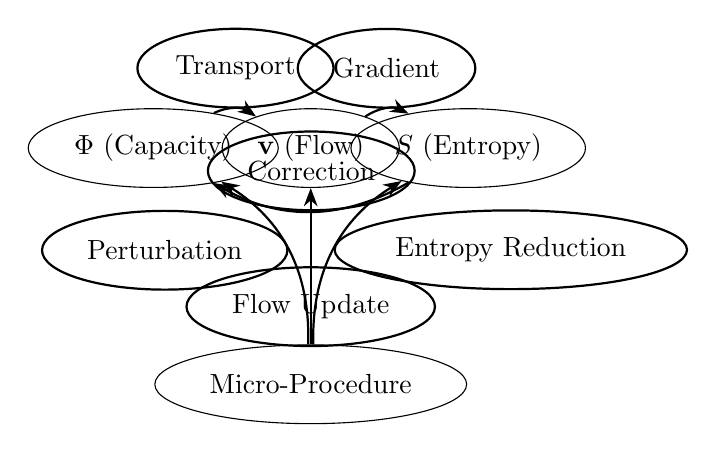
\begin{tikzpicture}[
  node distance=2cm,
  every node/.style={draw, ellipse, minimum height=1cm, minimum width=2cm, align=center},
  arrow/.style={-Stealth, thick}
]
\node (phi) {$\Phi$ (Capacity)};
\node (v) [right of=phi] {$\mathbf{v}$ (Flow)};
\node (s) [right of=v] {$S$ (Entropy)};
\node (proc) [below of=v, yshift=-1cm] {Micro-Procedure};
\draw[arrow] (phi) to [bend left] node[midway, above] {Transport} (v);
\draw[arrow] (v) to [bend left] node[midway, above] {Gradient} (s);
\draw[arrow] (s) to [bend left] node[midway, above] {Correction} (phi);
\draw[arrow] (proc) to [bend right] node[midway, left] {Perturbation} (phi);
\draw[arrow] (proc) to node[midway, below] {Flow Update} (v);
\draw[arrow] (proc) to [bend left] node[midway, right] {Entropy Reduction} (s);
\end{tikzpicture}
\caption{Knowledge graph for RSVP fields and Hepastitium micro-procedures. Arrows represent: Transport (\(\nabla \cdot (\mathbf{v} \Phi)\)), Gradient (\(\nabla \Phi, \nabla S\)), Correction (\(S_c - S\)), Perturbation (\(\delta \Phi_k\)), Flow Update (vector adjustments), Entropy Reduction (\(\Delta S_k\)).}
\label{fig:knowledge_graph}
\end{figure}

\subsection{Recursive Updates}
\label{subsec:recursive_updates}

Edge weights in \(\mathcal{G}\) update via Bayesian structure learning when entropy gradients exceed thresholds, ensuring adaptive causal inference.

\section{Conclusion}
\label{sec:conclusion}

Persistence is the capacity to metabolize entropy recursively across scales. RSVP unifies cosmology (space as plenum), biology (Hepastitium), architecture (xylomorphic cities), and cognition (semantic attractors), offering a paradigm for civilizational design. Future directions include empirical prototypes of Hepastitium relays, AI simulations obeying \(\mathcal{H}\)-balance, and ethical frameworks for hepatic governance.

\appendix

\section{Variational Derivation}
\label{app:variational}
A variational principle for \(\mathcal{H}\) is under development, ensuring \(\frac{dE}{dt} \le 0\) for systemic stability.

\section{Semantic Microscope Pseudocode}
\label{app:pseudocode}
\begin{verbatim}
function semanticMicroscope(G, query):
    results = []
    for node in G.nodes:
        if matches(query, node):
            results.append(traceCausalPath(G, node))
    return results
\end{verbatim}

\section{Entropic Empire Excerpt}
\label{app:entropic_empire}

\noindent\textbf{RSVP Turn Loop (JavaScript excerpt).}
\begin{verbatim}
// === RSVP Grid State ===
const W = 96, H = 64;                    // world dimensions
const N = W * H, at = (x,y)=>((y+H)%H)*W + ((x+W)%W);
let Phi = new Float32Array(N).fill(1.0); // scalar capacity Φ
let S   = new Float32Array(N).fill(0.5); // entropy field S
let Vx  = new Float32Array(N).fill(0.0); // vector flow v_x
let Vy  = new Float32Array(N).fill(0.0); // vector flow v_y

// Previous-step buffers (for ∂t terms)
let S_prev  = new Float32Array(N);
let Phi_prev= new Float32Array(N);

// === Parameters (tunable) ===
const dt = 1.0/6.0;      // turn time-step
const Sc = 0.45;         // entropy setpoint S_c
const lambda = 0.12;     // Φ feedback to S deviations
const kappa  = 0.08;     // S diffusion
const nuPhi  = 0.02;     // Φ diffusion (optional smoothing)
const nuV    = 0.04;     // v viscosity
const beta   = 0.30;     // advective nonlinearity
const xi     = 0.60;     // hepatic coupling into Φ
const eta    = 0.80;     // hepatic coupling out of S
const chi1   = 1.00, chi2 = 0.65, chi3 = 0.20; // hepatic weights

// === Utilities: finite differences ===
function grad(field, x, y) {
  const xm = at(x-1,y), xp = at(x+1,y), ym = at(x,y-1), yp = at(x,y+1);
  return {
    dx: 0.5*(field[xp]-field[xm]),
    dy: 0.5*(field[yp]-field[ym])
  };
}
function lap(field, x, y) {
  const c = at(x,y), xm=at(x-1,y), xp=at(x+1,y), ym=at(x,y-1), yp=at(x,y+1);
  return (field[xm]+field[xp]+field[ym]+field[yp]-4*field[c]);
}
function divV(x, y) {
  const gVx = grad(Vx, x, y), gVy = grad(Vy, x, y);
  return gVx.dx + gVy.dy;
}
function advectScalar(F, x, y) {
  // -∇·(v F) ≈ -(v·∇)F - F(∇·v)
  const c = at(x,y), gF = grad(F, x, y);
  const vdotGrad = Vx[c]*gF.dx + Vy[c]*gF.dy;
  return -vdotGrad - F[c]*divV(x,y);
}

// === Hepatic operator 𝓗[Φ,v,S] ===
function hepaticH(x, y) {
  const c = at(x,y);
  const gS = grad(S, x, y);
  const term1 = chi1*(gS.dx*Vx[c] + gS.dy*Vy[c]);   // (∇S·v)
  const term2 = -chi2*divV(x,y)*S[c];               // -(∇·v) S
  const dSdt  = (S[c] - S_prev[c]) / dt;            // ∂t S
  const term3 = chi3*dSdt;
  return term1 + term2 + term3;
}

// === Micro-procedure (hepastitium) hook ===
// Localized negentropic action: δΦ>0, ΔS<0 at (x,y)
function applyMicroProcedure(x, y, dPhi=0.02, dS=-0.02) {
  const c = at(x,y);
  Phi[c] = Math.max(0, Phi[c] + dPhi);
  S[c]   = Math.max(0, S[c]   + dS);
}

// Example scheduler stub: target voxels where S > threshold
function hepaticScheduler(threshold = 0.6, budget = 200) {
  for (let i = 0; i < budget; i++) {
    const x = (Math.random()*W)|0, y=(Math.random()*H)|0, c=at(x,y);
    if (S[c] > threshold) applyMicroProcedure(x,y);
  }
}

// === Turn update ===
function stepTurn() {
  // cache previous fields
  S_prev.set(S); Phi_prev.set(Phi);

  // 1) Run hepastitium scheduler (millions microsurgeries in real system)
  hepaticScheduler(0.62, 400);

  // 2) Field updates
  const Phi_next = new Float32Array(N);
  const S_next   = new Float32Array(N);
  const Vx_next  = new Float32Array(N);
  const Vy_next  = new Float32Array(N);

  for (let y=0; y<H; y++) for (let x=0; x<W; x++) {
    const c = at(x,y);

    // Φ_t+dt = Φ + dt[ -∇·(vΦ) + λ(S_c - S) + ξ 𝓗 + ν_Φ ∇²Φ ]
    const advPhi = advectScalar(Phi, x, y);
    const Hhep   = hepaticH(x, y);
    const dPhi   = advPhi + lambda*(Sc - S[c]) + xi*Hhep + nuPhi*lap(Phi, x, y);
    Phi_next[c]  = Math.max(0, Phi[c] + dt*dPhi);

    // v update (simplified Navier–Stokes-like with Φ pressure)
    const gPhi = grad(Phi, x, y);
    const vx   = Vx[c], vy = Vy[c];
    const advVx = -(vx*grad(Vx, x, y).dx + vy*grad(Vx, x, y).dy);
    const advVy = -(vx*grad(Vy, x, y).dx + vy*grad(Vy, x, y).dy);
    Vx_next[c] = vx + dt*( -gPhi.dx + advVx + nuV*lap(Vx, x, y) );
    Vy_next[c] = vy + dt*( -gPhi.dy + advVy + nuV*lap(Vy, x, y) );

    // S_t+dt = S + dt[ κ∇²S - η 𝓗 ]
    const dS = kappa*lap(S, x, y) - eta*Hhep;
    S_next[c] = Math.max(0, S[c] + dt*dS);
  }

  // 3) Commit
  Phi = Phi_next; S = S_next; Vx = Vx_next; Vy = Vy_next;

  // 4) Autosave summary (compress to means; full state optional)
  if ((performance.now()|0) % 5 === 0) {
    const mean = arr => arr.reduce((a,b)=>a+b,0)/arr.length;
    const snapshot = {
      t: Date.now(),
      Phi_mean: mean(Phi),
      S_mean:   mean(S),
      H_mean:   (()=>{ // average hepatic operator
        let h=0.0; for (let y=0;y<H;y++) for (let x=0;x<W;x++) h += hepaticH(x,y);
        return h / N;
      })()
    };
    localStorage.setItem("rsvp_autosave_summary", JSON.stringify(snapshot));
  }
}

// === Example tick ===
function tick(n=12) { for (let i=0;i<n;i++) stepTurn(); }
\end{verbatim}

\noindent\emph{Notes.}
(1) The hepatic operator \(\mathcal{H}\) implements the three-term definition
\((\nabla S\!\cdot\!\mathbf{v}) - (\nabla\!\cdot\!\mathbf{v})\,S + \partial_t S\),
scaled by \(\chi_{1,2,3}\).
(2) The scheduler stub demonstrates localized negentropic interventions
(\(\delta\Phi>0,\,\Delta S<0\)) when \(S\) exceeds a threshold; in a full build,
this is replaced by the Bayesian entropic scheduler.
(3) The autosave records coarse statistics, including the mean \(\mathcal{H}\),
so you can enforce the daily criterion \(\langle\mathcal{H}\rangle_\Omega \le 0\)
from Section~\ref{sec:empirical_validation}.

\section{Glossary}
\label{app:glossary}

\begin{description}[leftmargin=2em, labelwidth=1.5em, style=nextline]
  \item[\(\Phi\) (Scalar Capacity)] 
  Represents potential, vitality, or informational density within a region of the plenum.  It quantifies how much organized structure a system can sustain or generate.  In biological terms, \(\Phi\) measures functional reserve; in cognition, it corresponds to representational coherence; in cosmology, it maps to local capacity for negentropic formation.

  \item[\(\mathbf{v}\) (Vector Flow)] 
  Denotes directed transfer of energy, resources, or agents through the medium.  It governs advection and coupling between regions of differing capacity, linking microscopic and macroscopic coordination.  In cities, \(\mathbf{v}\) models logistics and data flux; in the body, circulation and signaling; in mind, streams of attention.

  \item[\(S\) (Entropy Field)] 
  Quantifies disorder, uncertainty, or informational loss.  \(S\) increases under diffusion and decreases under hepatic (repair) operations.  Its spatial gradients \(\nabla S\) drive restorative flows and define local thermodynamic stress within the plenum.

  \item[\(\mathcal{H}[\Phi,\mathbf{v},S]\) (Hepatic Operator)] 
  A functional converting entropy flow into negentropic correction:
  \[
  \mathcal{H} = \chi_1(\nabla S\!\cdot\!\mathbf{v}) 
               - \chi_2(\nabla\!\cdot\!\mathbf{v})\,S
               + \chi_3\,\frac{\partial S}{\partial t}.
  \]
  Negative values indicate regenerative absorption of disorder; positive values indicate entropy emission or decay.

  \item[\(S_c\) (Critical Entropy)] 
  Reference equilibrium level toward which hepatic regulation drives \(S\).  In biology, \(S_c\) corresponds to optimal metabolic disorder—enough fluctuation for adaptability but not enough to destabilize structure.

  \item[\(\lambda, \kappa, \xi, \eta\)] 
  Coupling coefficients.  \(\lambda\) mediates scalar–entropy feedback, \(\kappa\) governs entropy diffusion, \(\xi\) and \(\eta\) control hepatic influence on \(\Phi\) and \(S\) respectively.

  \item[\(\langle \mathcal{H} \rangle_\Omega \le 0\) (Longevity Condition)] 
  Global criterion for regenerative equilibrium: the average hepatic operator over domain \(\Omega\) must be non-positive, ensuring that entropy is reabsorbed faster than it accumulates.

  \item[Hepastitium] 
  Contraction of \emph{hepatostitium} (from Greek \emph{hepar}, “liver,” and Latin \emph{stitium}, “standing-place”).  Denotes the endogenous tissue-sampling and microsurgical relay network maintaining systemic coherence through continuous entropy management.

  \item[Xylomorphic Architecture] 
  Design paradigm modeling cities and ecosystems after forest metabolisms.  Converts waste flows into regenerative feedback, treating infrastructure as a macroscopic hepatic organ.

  \item[Proof-of-Useful-Work-and-Heat] 
  Thermodynamic governance model in which computation and heating jointly satisfy ecological and informational needs, aligning human infrastructure with entropic reciprocity.

  \item[Yarncrawler] 
  Mesoscale autonomous repair framework that extends hepatic recursion to infrastructures and semantic systems via trajectory-aware agents performing distributed maintenance.

  \item[Semantic Microscope] 
  Knowledge-graph and inference engine mapping micro-procedures, field variables, and causal efficiencies.  Supports recursive exploration and optimization of negentropic interventions.

  \item[\(\Phi_c\)-Coherence Index] 
  Empirical measure of scalar-field alignment:
  \(\Phi_c = 1 - \mathrm{Var}(\Phi_i)/\langle \Phi_i\rangle\).  
  High \(\Phi_c\) indicates coordinated capacity and cognitive or physiological stability.

  \item[Negentropic Flux Score (NFS)] 
  Integral measure of entropy absorption efficiency:
  \(\mathrm{NFS} = \frac{1}{T}\int_0^T\!\!\int_\Omega(\eta\nabla^2 S - \xi\mathcal{H})\,dV\,dt.\)
  Negative or near-zero NFS implies regenerative balance; positive NFS denotes net entropy leakage.

  \item[Regenerative Equilibrium] 
  The dynamic steady state in which systemic entropy remains bounded through continuous hepatic recursion—biological longevity, cognitive continuity, and civilizational sustainability all correspond to maintaining this equilibrium.
\end{description}

\bibliographystyle{plain}
\begin{thebibliography}{9}
\bibitem{prigogine1977} Prigogine, I., \emph{Time, Structure and Fluctuations}, 1977.
\bibitem{schrodinger1944} Schrödinger, E., \emph{What is Life?}, 1944.
\bibitem{friston2010} Friston, K., \emph{The Free-Energy Principle}, 2010.
\bibitem{ortega1930} Ortega y Gasset, J., \emph{The Revolt of the Masses}, 1930.
\bibitem{spinoza1677} Spinoza, B., \emph{Ethics}, 1677.
\end{thebibliography}

\end{document}